\documentclass{article}
\usepackage{tikz}
\usetikzlibrary{shapes.geometric, arrows}

\begin{document}
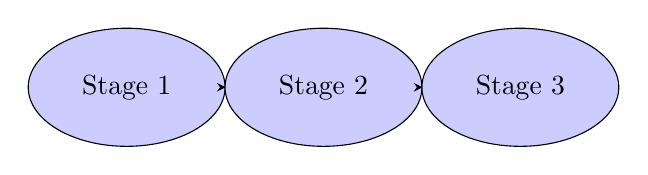
\begin{tikzpicture}[node distance=2.5cm, >=stealth]

    % Define the styles for the nodes
    \tikzstyle{stage} = [ellipse, draw, fill=blue!20, text centered, minimum width=2.5cm, minimum height=1.5cm]
    
    % Nodes
    \node (stage1) [stage] {Stage 1};
    \node (stage2) [stage, right of=stage1] {Stage 2};
    \node (stage3) [stage, right of=stage2] {Stage 3};
    
    % Arrows
    \draw[<-] (stage1) -- (stage2);
    \draw[<-] (stage2) -- (stage3);
    
    \end{tikzpicture}
\end{document}
